\vspace{-0.5em}
\section{Experiments}
\vspace{-0.5em}

\subsection{Experiment Settings}

\textbf{Implementation details}. We implement our listening-head generator with a latent flow-matching transformer and train it with mixed precision using Accelerate on 4$\times$L40s GPUs. We use AdamW (lr=5e-4), gradient clipping (1.0), cosine decay with warmup, batch size 256, and train for 650 epochs. 
The default temporal setup is 25 FPS, and audio is sampled at 16 kHz. Input frames are resized to 512$\times$512 and normalized to \([-1,1]\). 
We split the train/test set into a ratio 9:1. 
The pretrained motion autoencoder \cite{wang2022lia} and audio LLM \cite{Qwen2-Audio} are kept frozen. 
More details can be found in Appendix \ref{app:architecture_optimization}.

\textbf{Evaluation metrics}. We use Fréchet Inception Distance (\textbf{FID}) \cite{Seitzer2020FID} and 16-frame Fréchet Video Distance (\textbf{FVD}) \cite{unterthiner2018fvd} to assess image and video generation quality; Peak Signal-to-Noise Ratio (\textbf{PSNR}) for measuring pixel fidelity; Structural Similarity Index (\textbf{SSIM}) for perceived change in structural information; Variation (\textbf{Var}) \cite{ng2022learning} for motion diversity and richness; Learned Perceptual Image Patch Similarity (\textbf{LPIPS}) \cite{zhang2018lpips} for measuring perceptual distance; Residual Pearson Correlation Coefficient (\textbf{rPCC}) to measure the correlation between motions of speaker and listener; \textbf{DI-Sync} \cite{pan2026interdyad} to quantify the causal coordination between the speaker’s verbal cues and the listener’s non-verbal responses. We also use metrics proposed in Sec. \ref{sec:metric} (i.e., \textbf{R-F1}, \textbf{R-tIoU}, \textbf{R-ATD}, and \textbf{R-FID}) to specifically evaluate the accuracy and generation quality of reactions.

\textbf{Comparison methods}. We choose L2L \cite{ng2022learning}, DIM \cite{tran2024dim}, ViCo \cite{zhou2022vico}, ListenFormer \cite{liu2024listenformer}, and DyStream \cite{chen2025dystream} for comparison. All methods are trained and tested using our dataset, respectively.



\subsection{Experiment Results}

\textbf{Quantitative comparison with SOTA methods}. We compare our method with prior approaches on the RealTalk and Seamless in Table \ref{tab:quant_results} (The bold are the best, while the underlined are the second best). On RealTalk, our method achieves the best overall performance across most metrics, improving both visual quality and reaction modeling. Lower FID/FVD and LPIPS indicate better perceptual realism and temporal coherence, while higher DI-Sync, R-F1, and R-tIoU, together with lower R-ATD, show more accurate and temporally aligned listener reactions. On the more challenging Seamless subset, our method maintains strong visual fidelity and consistently improves reaction-related metrics, especially R-F1, R-tIoU, and R-FID. Although DyStream obtains slightly higher Var, our method provides a better balance between motion diversity, reaction accuracy, and visual quality.



\begin{table*}[t]
    \centering
    \fontsize{7.2pt}{6pt}\selectfont
    \setcellgapes{1.2pt}
    \makegapedcells
    \setlength{\tabcolsep}{1.5pt}
    \caption{Quantitative comparison of state-of-the-art methods on the RealTalk and Seamless datasets}
    \vspace{-0.5em}
    \label{tab:quant_results}
    \begin{tabular}{l|l|cccccccc|cccc}
        \Xhline{1.2pt}
        
        Dataset
        & Method 
        & PSNR $\uparrow$ 
        & SSIM $\uparrow$ 
        & FID $\downarrow$ 
        & FVD $\downarrow$ 
        & Var $\uparrow$ 
        & LPIPS $\downarrow$ 
        & rPCC $\downarrow$ 
        & DI-Sync $\uparrow$ 
        & R-F1 $\uparrow$ 
        & R-tIoU $\uparrow$ 
        & R-ATD $\downarrow$ 
        & R-FID $\downarrow$ \\
        
        \hline
        
        \multirow{6}{*}{\raisebox{-2\height}{RealTalk}}
        & L2L 
        & 14.684 & 0.575 & 45.782 & 202.798 & 1.885 & 0.637 & 0.323 & 0.182 & 0.454 & 0.505 & 78.265 & 24.683 \\
        
        & DIM 
        & 16.223 & 0.495 & 37.717 & 188.266 & 2.765 & 0.585 & 0.289 & 0.190 & \smash{\uline{0.576}} & 0.551 & 133.082 & 22.971 \\
        
        & ViCo 
        & 14.932 & \smash{\uline{0.602}} & 44.089 & 185.040 & 2.560 & 0.579 & 0.261 & 0.178 & 0.429 & 0.572 & 92.454 & 26.105 \\
        
        & ListenFormer 
        & 17.454 & 0.582 & \smash{\uline{36.173}} & 165.290 & 1.625 & 0.525 & 0.256 & \smash{\uline{0.221}} & 0.334 & 0.650 & 73.379 & 23.097 \\
        
        & DyStream 
        & 17.894 & \textbf{0.611} & 37.416 & \smash{\uline{147.537}} & \smash{\uline{2.802}} & \smash{\uline{0.467}} & \smash{\uline{0.248}} & 0.208 & 0.535 & \smash{\uline{0.694}} & \smash{\uline{63.171}} & \smash{\uline{15.337}} \\

        & Ours
        & \textbf{17.972} & 0.601 & \textbf{35.697} & \textbf{142.454} & \textbf{2.916} & \textbf{0.454} & \textbf{0.227} & \textbf{0.245} & \textbf{0.594} & \textbf{0.704} & \textbf{57.388} & \textbf{15.192} \\
        
        \hline
        
        \multirow{6}{*}{\raisebox{-2\height}{Seamless}}
        & L2L 
        & 11.634 & 0.456 & 36.287 & 245.885 & 1.481 & 0.542 & 0.372 & 0.192 & 0.409 & \smash{\uline{0.554}} & 112.938 & 35.697 \\
        
        & DIM 
        & 12.856 & 0.391 & 29.885 & 289.695 & 2.180 & 0.411 & 0.398 & 0.172 & 0.296 & 0.501 & 157.302 & 34.379 \\
        
        & ViCo 
        & 12.830 & 0.458 & 34.932 & 230.037 & 2.021 & 0.449 & 0.385 & 0.165 & 0.389 & 0.523 & 140.344 & 37.926 \\
        
        & ListenFormer 
        & \smash{\uline{13.824}} & \smash{\uline{0.464}} & \smash{\uline{28.662}} & 210.474 & 1.287 & 0.472 & 0.361 & \textbf{0.212} & 0.369 & 0.511 & 128.705 & 35.266 \\
        
        & DyStream 
        & 13.664 & \smash{\uline{0.464}} & 31.755 & \smash{\uline{209.876}} & \textbf{2.452} & \smash{\uline{0.409}} & \smash{\uline{0.329}} & 0.202 & \smash{\uline{0.414}} & 0.553 & \smash{\uline{110.808}} & \smash{\uline{30.774}} \\

        & Ours
        & \textbf{14.245} & \textbf{0.473} & \textbf{27.288} & \textbf{193.281} & \smash{\uline{2.447}} & \textbf{0.371} & \textbf{0.301} & \smash{\uline{0.205}} & \textbf{0.460} & \textbf{0.582} & \textbf{102.113} & \textbf{28.857} \\
        
        \Xhline{1.2pt}
    \end{tabular}
    \vspace{-1.7em}
\end{table*}


\textbf{Per-class reaction evaluation comparison with DyStream}. Table \ref{tab:per_class_results} further reports per-class reaction evaluation. The results reveal some category-dependent difficulties: large-amplitude reactions such as \textit{laughing} are easier to detect and temporally align, while subtle motions such as \textit{nodding} and \textit{head shaking} are more sensitive to timing errors. \textit{Surprised} remains the most challenging category due to its ambiguity and sparsity, whereas \textit{smiling} achieves more balanced performance benefiting from its larger data scale. Overall, Seamless yields consistently lower scores than RealTalk, reflecting its greater diversity and complexity.

\begin{table}[t]
    \centering
    \fontsize{7.5pt}{6.5pt}\selectfont
    \setcellgapes{1.2pt}
    \makegapedcells
    \setlength{\tabcolsep}{1.5pt} 
    \caption{Per-class reaction comparison between Dystream and our method with proposed metrics}
    \vspace{0.1em}
    \label{tab:per_class_results}
    \begin{tabular}{c|l|c|cc|cc|cc|cc}
        \Xhline{1.2pt}
        
        \multirow{2}{*}{Dataset} & \multirow{2}{*}{Reaction} & \multirow{2}{*}{\makecell[c]{Data\\Amount}} & \multicolumn{2}{c|}{R-F1 $\uparrow$} & \multicolumn{2}{c|}{R-tIoU $\uparrow$} & \multicolumn{2}{c|}{R-ATD $\downarrow$} & \multicolumn{2}{c}{R-FID $\downarrow$} \\
        
        \cline{4-11}
        
        & & & Dystream & Ours & Dystream & Ours & Dystream & Ours & Dystream & Ours \\
        
        \hline

        \multirow{6}{*}{\raisebox{-3\height}{RealTalk}}
        & \textit{nodding}        & 3033 & 0.562 & \textbf{0.602} & 0.672 & \textbf{0.686} & 66.168 & \textbf{60.375} & 15.114 & \textbf{14.680} \\
        & \textit{head shaking}   & 3588 & 0.521 & \textbf{0.581} & \textbf{0.655} & 0.652 & 67.447 & \textbf{61.894} & 15.626 & \textbf{15.316} \\
        & \textit{smiling}        & 4804 & 0.554 & \textbf{0.633} & 0.718 & \textbf{0.753} & 60.396 & \textbf{54.882} & 14.883 & \textbf{14.371} \\
        & \textit{laughing}       & 2397 & 0.569 & \textbf{0.656} & 0.735 & \textbf{0.769} & 57.026 & \textbf{48.189} & 16.005 & \textbf{15.697} \\
        & \textit{frowning}       & 2745 & 0.511 & \textbf{0.549} & 0.705 & \textbf{0.707} & 61.518 & \textbf{54.793} & \textbf{15.010} & 15.024 \\
        & \textit{surprised}      & 1860 & 0.503 & \textbf{0.540} & \textbf{0.679} & 0.658 & 66.515 & \textbf{64.233} & \textbf{15.397} & 16.007 \\
        \hline

        \multirow{6}{*}{\raisebox{-3\height}{Seamless}}
        & \textit{nodding}        & 7197  & 0.426 & \textbf{0.476} & 0.535 & \textbf{0.548} & 114.168 & \textbf{110.223} & 30.294 & \textbf{27.908} \\
        & \textit{head shaking}   & 9202  & 0.405 & \textbf{0.450} & 0.515 & \textbf{0.522} & 116.043 & \textbf{110.930} & 31.054 & \textbf{28.445} \\
        & \textit{smiling}        & 10963 & 0.438 & \textbf{0.501} & 0.582 & \textbf{0.617} & 104.982 & \textbf{96.309}  & 30.038 & \textbf{28.638} \\
        & \textit{laughing}       & 5923  & 0.455 & \textbf{0.515} & 0.595 & \textbf{0.636} & 100.529 & \textbf{91.165}  & 31.645 & \textbf{29.887} \\
        & \textit{frowning}       & 7241  & 0.392 & \textbf{0.424} & 0.564 & \textbf{0.601} & 107.388 & \textbf{98.237}  & 29.885 & \textbf{27.424} \\
        & \textit{surprised}      & 5604  & 0.373 & \textbf{0.409} & 0.528 & \textbf{0.575} & 121.848 & \textbf{106.038} & 31.744 & \textbf{30.856} \\
        
        \Xhline{1.2pt}
    \end{tabular}
    \vspace{-2em}
\end{table}




\textbf{Qualitative comparisons on RealTalk}. Fig. \ref{fig:realtalk} shows two representative qualitative results on RealTalk, where we uniformly sample the same set of frames for each method to compare. Existing methods often generate static listeners (L2L, DIM, ViCo) or reactions with inaccurate timing (ListenFormer, DyStream). In contrast, our method produces more expressive and contextually consistent reactions that better match the ground truth in both type and timing, demonstrating improved modeling of listener reactions. Qualitative results of Seamless are provided in Appendix \ref{sec:appendix-seamless}.

\begin{figure}[t]
    \centering
    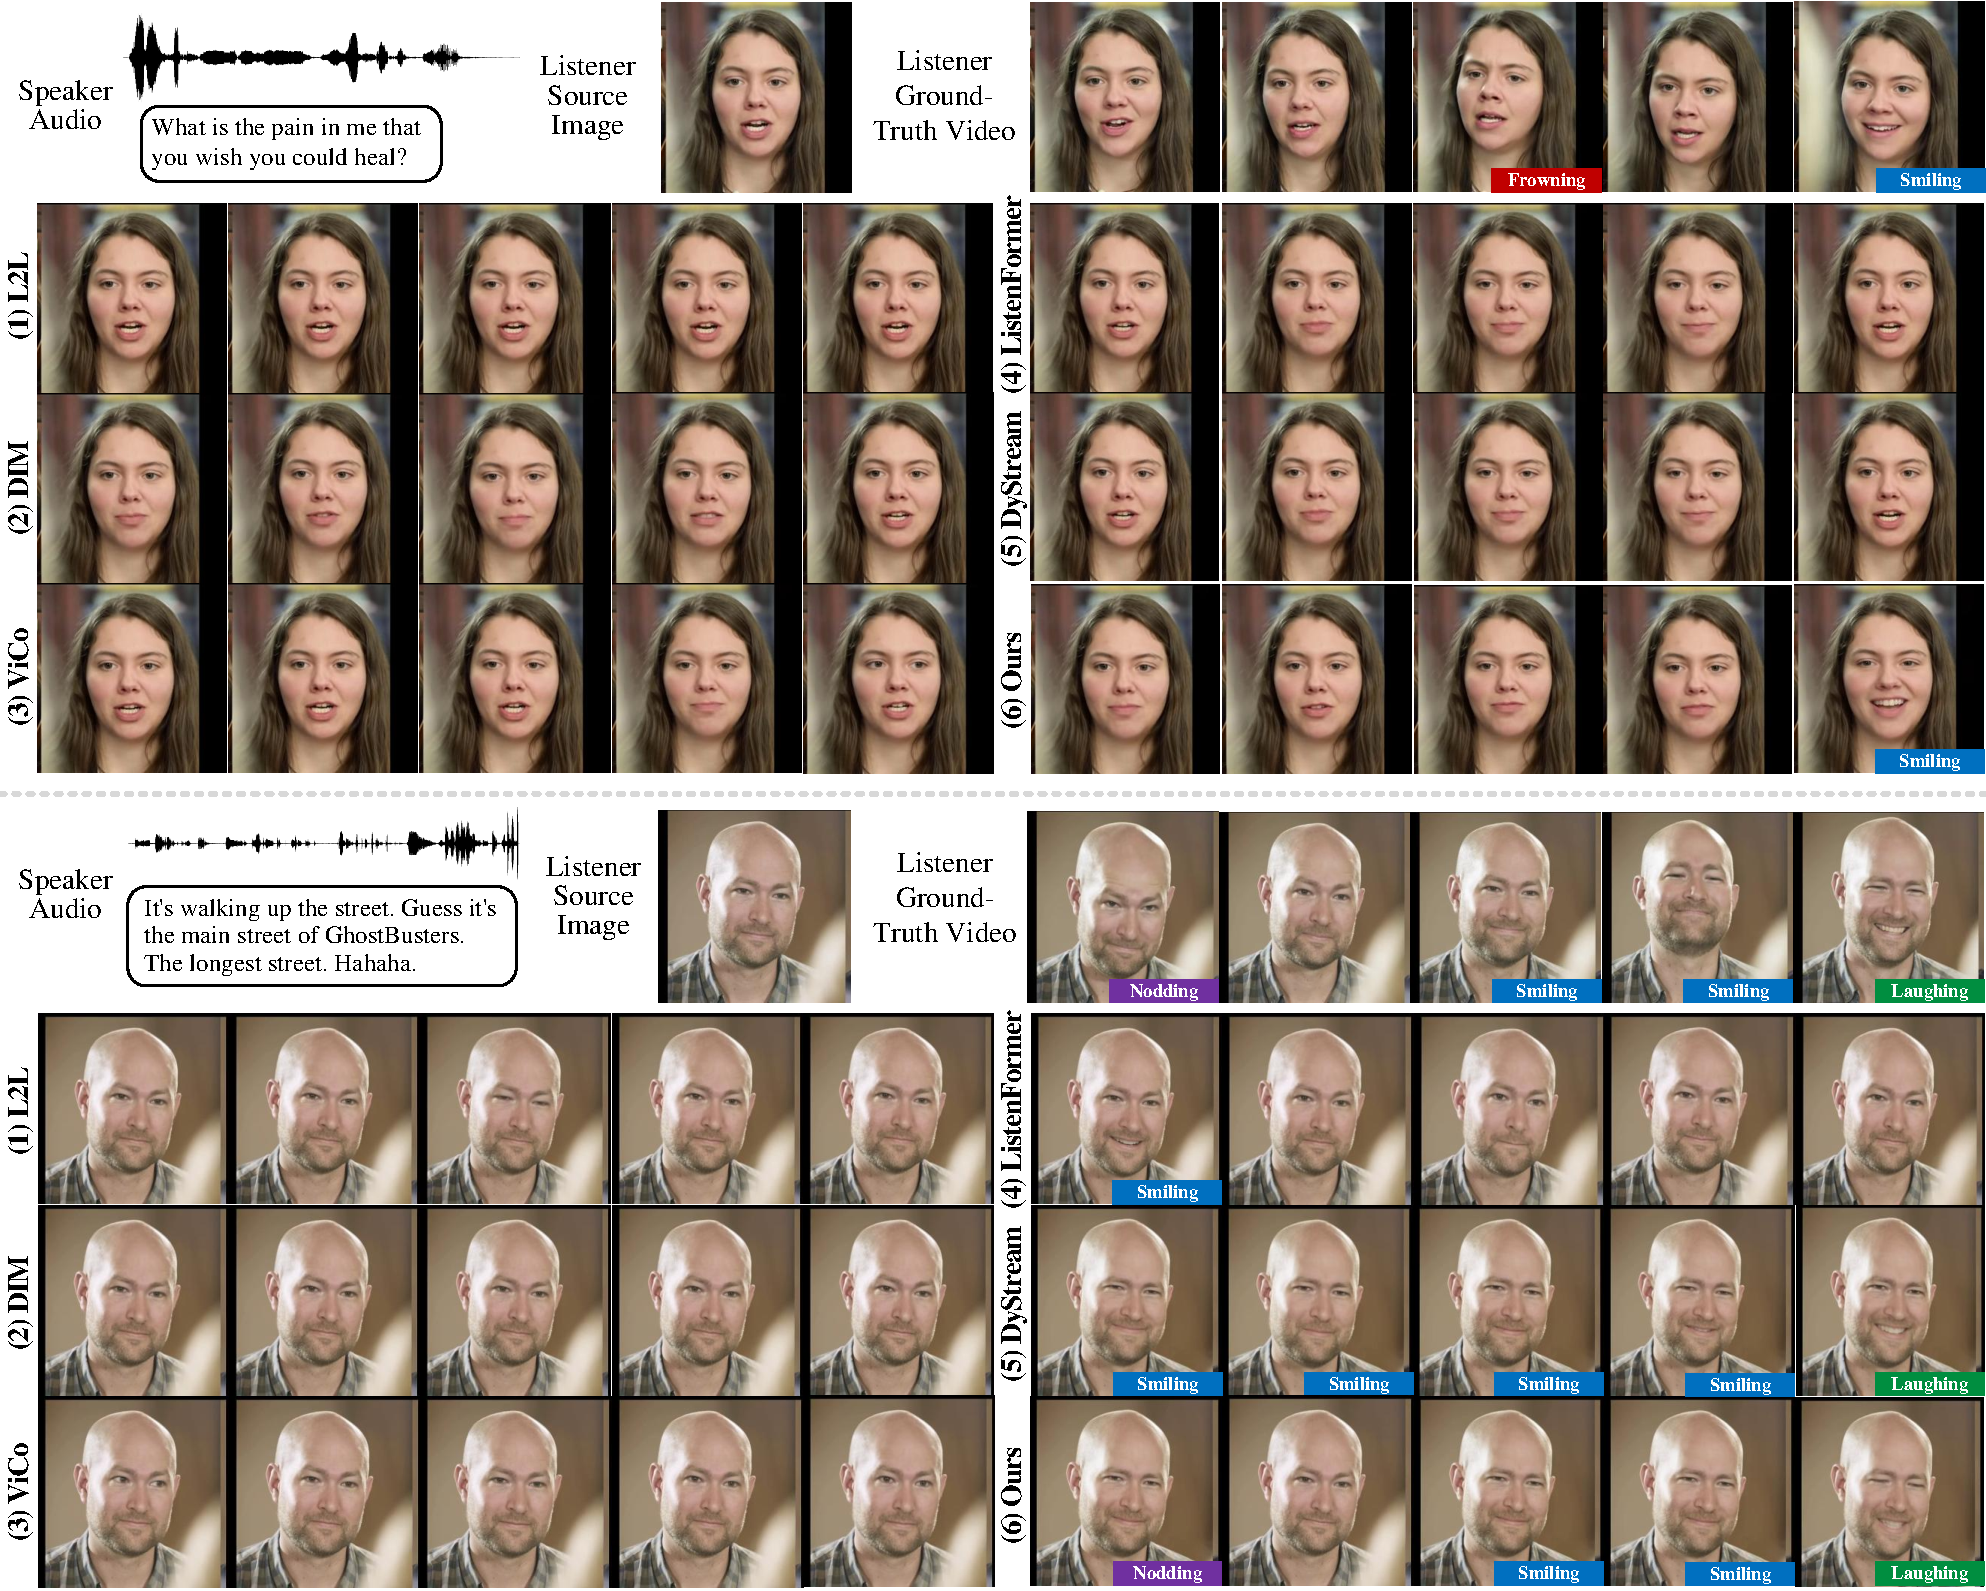
\includegraphics[width=\linewidth,keepaspectratio]{files/result_realtalk.pdf}
    \vspace{-1.5em}
    \caption{Qualitative comparison of our approach with state-of-the-art methods on the RealTalk dataset. Reaction labels are displayed at frames where reactions are detected.
    Our method generates more natural listening motions and reactions that are more temporally aligned with the ground truths than other methods.}
    \label{fig:realtalk}
    \vspace{-1em}
\end{figure}

% We include qualitative results of Seamless in Appendix \ref{sec:appendix-seamless}.



\textbf{Human evaluation and reaction appropriateness}. We conduct a human evaluation to assess the naturalness, contextual appropriateness, and timing plausibility of generated reactions. We sample 100 generated videos from the RealTalk test set (15.94s on average), containing 165 reaction events. We recruit 23 participants (4 undergraduate, 13 master's, and 6 PhD students; mean age 23; 18 male and 5 female). Given the speaker audio and transcript used as model context, participants evaluate each detected reaction event, including its type and start/end times, using three binary criteria: whether the motion appears natural, the reaction is appropriate to the speaker context, and it occurs at plausible time. This yields $165\times23=3{,}795$ reaction-participant annotations. We compute the Human Agreement Rate (HAR) for each criterion as the proportion of reactions judged positively (e.g., $\mathrm{HAR}_{\text{naturalness}}=\#\text{natural judgments}\ /\ \#\text{all judgments}$), where higher HAR indicates better alignment with human judgment. The 165 events comprise 41 nodding, 14 head-shaking, 29 smiling, 35 laughing, 26 frowning, and 20 surprised reactions. Table \ref{tab:human_evaluation} reports participant-averaged HAR for each reaction type, with the overall score computed as the average across the six categories.

% \vspace{-1em}
\begin{table}[t]
    \centering
    \fontsize{9pt}{7.5pt}\selectfont
    \setcellgapes{2pt}
    \makegapedcells
    \setlength{\tabcolsep}{2pt}
    \caption{Human evaluation results across different reaction categories.}
    \label{tab:human_evaluation}
    \begin{tabular}{c|c|c|c}
        \Xhline{1.2pt}
        Reaction & Reaction Naturalness & Contextual Appropriateness & Timing Plausibility \\
        \hline
        \textit{nodding} & 0.954 & 0.975 & 0.982 \\
        \textit{head shaking} & 0.969 & 0.914 & 0.937 \\
        \textit{smiling} & 0.897 & 0.868 & 0.944 \\
        \textit{laughing} & 0.852 & 0.836 & 0.955 \\
        \textit{frowning} & 0.902 & 0.874 & 0.884 \\
        \textit{surprised} & 0.824 & 0.898 & 0.905 \\
        \Xhline{0.5pt}
        \textbf{Overall} & \textbf{0.899} & \textbf{0.894} & \textbf{0.935} \\
        \Xhline{1.2pt}
    \end{tabular}
    \vspace{-2em}
\end{table}

% As shown in the table, our generated reactions achieve high HARs across all dimensions, with 89.9\%, 89.4\%, and 93.5\% agreement on reaction naturalness, contextual appropriateness, and timing plausibility, respectively, validating the quality of generated reactions via our method. Notably, the timing plausibility achieves the highest score, proving the effectiveness of our temporal reaction modeling. Meanwhile, more challenging expressive reactions such as ``laughing'' and ``surprised'' receive relatively lower motion scores, suggesting that these reactions remain challenging due to complex facial dynamics. Furthermore, the relatively lower contextual appropriateness for laughing indicates that laughter requires a deeper understanding of conversational semantics and social context. Compared with simple agreement behaviors such as nodding, laughter is often triggered by subtle cues such as humor, emotion, and interpersonal interaction, making it inherently more challenging to generate appropriately.

As shown in Table \ref{tab:human_evaluation}, our method achieves high HARs of 89.9\%, 89.4\%, and 93.5\% for reaction naturalness, contextual appropriateness, and timing plausibility, respectively. The strong timing score supports the effectiveness of our temporal modeling. More expressive reactions, such as \textit{laughing} and \textit{surprised}, remain more challenging due to complex facial dynamics, while the relatively lower contextual appropriateness of laughter highlights its dependence on subtle semantic and social cues, including humor, emotion, and interpersonal interaction.




\vspace{-0.5em}
\subsection{Ablation Study}
\vspace{-0.5em}

We conduct our ablation studies on RealTalk dataset. More ablation studies, including speaker audio length, prosody channel projection, and reaction loss type, are included in appendix \ref{sec:appendix-ablation}

\textbf{Module effectiveness}. 
We ablate the effectiveness of the prosody conditioning mechanism and temporal reaction loss in Table \ref{tab:ablation_modules}. It can be seen that, adding the prosody condition improves visual quality and motion dynamics (e.g., PSNR, FVD, Var), but brings limited gains on reaction-related metrics and even degrades temporal precision (R-ATD), indicating that prosodic cues alone are insufficient for accurate reaction modeling. 
In contrast, the reaction loss yields substantial improvements across various metrics (DI-Sync, R-F1, R-tIoU) and significantly reduces R-ATD and R-FID, demonstrating its key role in learning temporally aligned and semantically correct reactions. Combining both modules achieves the best overall performance, showing that prosody provides complementary temporal cues on top of explicit reaction supervision.

\textbf{Reaction loss coefficient $\lambda_{\text{react}}$}. Table \ref{tab:ablation_coef} shows that increasing the reaction loss coefficient $\lambda_{\text{react}}$ from a small value (0.01) to a moderate range (0.05--0.1) consistently improves both visual quality and reaction-related metrics, indicating that stronger supervision helps the model learn more accurate and temporally aligned behaviors. However, further increasing $\lambda_{\text{react}}$ (e.g., $\geq$ 0.2) leads to degraded performance in both generation quality and reaction accuracy, suggesting that overly strong supervision disrupts the balance between the two objectives. Overall, $\lambda_{\text{react}}$=0.05 achieves the best trade-off across metrics.

\textbf{Effectiveness of prosody conditioning}. We further analyze the effect of prosody conditioning at the reaction level in Table \ref{tab:prosody_conditioning}, reporting percentage changes for clarity. Prosody conditioning consistently improves R-F1 across all reaction types, with the largest gain for \textit{laughing}, suggesting that speaker prosodic changes provide useful cues for reaction expressiveness. However, it does not consistently improve temporal metrics: most reaction categories show degraded R-tIoU and R-ATD. This is likely because prosody reflects the speaker's affective state but does not explicitly determine whether or when a listener should react; relying too strongly on prosodic changes may therefore trigger reactions too immediately, whereas real conversational responses also depend heavily on semantic and contextual cues. Our temporal reaction loss complements prosody conditioning by explicitly supervising reaction occurrence and timing.

% We further analyze the effect of prosody conditioning at the reaction level in Table \ref{tab:prosody_conditioning}. We display the corresponding percentage changes and highlight those improvements. Prosody conditioning can effectively improve R-F1 for each reaction, especially ``laughing''. This is because reactions are relatively associated with and triggered by prosodic changes from the speaker, where our prosody conditioning mechanism helps to identify those changes.

% Although prosody conditioning improves reaction expressiveness, it does not consistently improve R-tIoU or reduce R-ATD as the reviewer identified. Nearly all reaction categories experience evident performance drops in R-tIoU and R-ATD, and one reason is that prosody reflects the speaker's affective state but does not explicitly determine whether and when the listener should react. Prosody conditioning tends to make the model output reactions right after prosodic changes from speakers, which is somewhat different compared to real conversations, because reactions are not only associated with prosody but also heavily with conversational contexts. In our work, temporal reaction loss plays a complementary role by providing supervision for the model to learn reaction occurrence and timing.


\begin{table*}[t]
    \centering
    \caption{Ablation of the proposed components and sensitivity to the reaction loss coefficient}
    \vspace{-0.5em}
    \label{tab:ablation_combined}

    \begin{subtable}{\textwidth}
        \centering
        \fontsize{7.2pt}{7pt}\selectfont
        \setcellgapes{2pt}
        \makegapedcells
        \setlength{\tabcolsep}{2pt}
        \caption{Ablation study of the prosody conditioning and the temporal reaction loss}
        \vspace{-0.5em}
        \label{tab:ablation_modules}
        \begin{tabular}{cc|cccccccc|cccc}
            \Xhline{1.2pt}
            \multicolumn{2}{c|}{Modules} & \multicolumn{12}{c}{Metrics} \\
            \hline
            \multirow{2}{*}{\makecell[c]{Prosody\\Cond.}} 
                & \multirow{2}{*}{\makecell[c]{Reaction\\Loss}}
                & \multirow{2}{*}{PSNR $\uparrow$}
                & \multirow{2}{*}{SSIM $\uparrow$}
                & \multirow{2}{*}{FID $\downarrow$}
                & \multirow{2}{*}{FVD $\downarrow$}
                & \multirow{2}{*}{Var $\uparrow$}
                & \multirow{2}{*}{LPIPS $\downarrow$}
                & \multirow{2}{*}{rPCC $\downarrow$}
                & \multirow{2}{*}{DI-Sync $\uparrow$}
                & \multirow{2}{*}{R-F1 $\uparrow$}
                & \multirow{2}{*}{R-tIoU $\uparrow$}
                & \multirow{2}{*}{R-ATD $\downarrow$}
                & \multirow{2}{*}{R-FID $\downarrow$} \\
            & & & & & & & & & & & & & \\
            \hline
            -- & -- 
                & 13.113 & 0.534 & 43.286 & 188.044 & 1.862 & 0.749 
                & 0.283 & 0.178 & 0.404 & 0.599 & 89.984 & 23.706 \\
            \checkmark & -- 
                & 14.071 & 0.558 & 40.798 & 159.745 & 2.206 & 0.659 
                & 0.274 & 0.194 & 0.481 & 0.574 & 100.342 & 20.603 \\
            -- & \checkmark 
                & \smash{\uline{17.212}} & \smash{\uline{0.586}} & \smash{\uline{36.635}} & \smash{\uline{145.858}} & \smash{\uline{2.896}} & \smash{\uline{0.477}} 
                & \smash{\uline{0.252}} & \smash{\uline{0.236}} & \smash{\uline{0.579}} & \smash{\uline{0.695}} & \textbf{55.657} & \smash{\uline{17.885}} \\
            \checkmark & \checkmark 
                & \textbf{17.973} & \textbf{0.601} & \textbf{35.691} & \textbf{142.456} & \textbf{2.913} & \textbf{0.454} 
                & \textbf{0.227} & \textbf{0.245} & \textbf{0.594} & \textbf{0.704} & \smash{\uline{57.386}} & \textbf{15.192} \\
            \Xhline{1.2pt}
        \end{tabular}
    \end{subtable}

    \vspace{0.6em}

    \begin{subtable}{\textwidth}
        \centering
        \fontsize{7.5pt}{6.8pt}\selectfont
        \setcellgapes{2pt}
        \makegapedcells
        \setlength{\tabcolsep}{2pt}
        \caption{Effect of varying the temporal reaction loss coefficient $\lambda_{\text{react}}$}
        \vspace{-0.5em}
        \label{tab:ablation_coef}
        \begin{tabular}{c|cccccccc|cccc}
            \Xhline{1.2pt}
            \multirow{2}{*}{\makecell[c]{Reaction\\Loss Coef.}} 
            & \multicolumn{12}{c}{Metrics} \\
            \cline{2-13}
            & PSNR $\uparrow$
            & SSIM $\uparrow$
            & FID $\downarrow$
            & FVD $\downarrow$
            & Var $\uparrow$
            & LPIPS $\downarrow$
            & rPCC $\downarrow$
            & DI-Sync $\uparrow$
            & R-F1 $\uparrow$
            & R-tIoU $\uparrow$
            & R-ATD $\downarrow$
            & R-FID $\downarrow$ \\
            \hline
            0.01 
            & 15.446 & 0.573 & 37.034 & 178.878 & 1.848 & 0.502 
            & 0.232 & 0.196 & 0.572 & 0.606 & 78.672 & 17.976 \\
            \textbf{0.05} 
            & \textbf{17.973} & 0.601 & \textbf{35.691} & \textbf{142.456} & \textbf{2.913} & \smash{\uline{0.454}} 
            & \textbf{0.227} & \textbf{0.245} & 0.594 & \smash{\uline{0.704}} & \textbf{57.386} & \textbf{15.192} \\
            0.1 
            & 17.904 & \textbf{0.632} & 36.147 & \smash{\uline{144.895}} & \smash{\uline{2.901}} & \textbf{0.447} 
            & \smash{\uline{0.230}} & 0.223 & \textbf{0.613} & \textbf{0.711} & \smash{\uline{64.790}} & 16.326 \\
            0.2 
            & \smash{\uline{17.566}} & \smash{\uline{0.610}} & \smash{\uline{36.032}} & 149.286 & 2.744 & 0.471 
            & 0.245 & \smash{\uline{0.230}} & \smash{\uline{0.602}} & 0.684 & 69.131 & 15.875 \\
            0.5 
            & 15.297 & 0.595 & 39.115 & 163.477 & 2.331 & 0.502 
            & 0.248 & 0.205 & 0.582 & 0.695 & 77.437 & \smash{\uline{15.548}} \\
            1 
            & 15.132 & 0.560 & 42.855 & 169.964 & 1.948 & 0.545 
            & 0.261 & 0.210 & 0.549 & 0.663 & 78.551 & 17.036 \\
            \Xhline{1.2pt}
        \end{tabular}
    \end{subtable}

    \vspace{-1.5em}
\end{table*}